%!TEX root = ./template-skripsi.tex
%-------------------------------------------------------------------------------
%                            BAB III
%               			PEMBAHASAN
%-------------------------------------------------------------------------------

\chapter{METODOLOGI PENELITIAN}

\section{Deskripsi Penelitian}

Aplikasi yang akan dibuat pada penelitian ini adalah aplikasi pendukung teknologi perikanan modern. Aplikasi berfungsi untuk mencatat setiap kegiatan yang dilakukan oleh petani ikan air tawar selama masa budidaya berlangsung. Selain hal tersebut, aplikasi ini juga dapat mengukur \textit{Food Conversion Ratio} dari setiap musim budidaya yang diselesaikan oleh petani. 

\section{Desain Penelitian}

\begin{figure}[H]
	\centering
	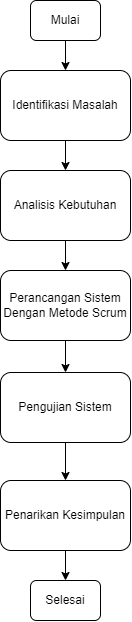
\includegraphics[keepaspectratio, width=2cm]{gambar/tahapan}
	\caption{Tahapan Penelitian}
	\label{gambar:tahapan}
\end{figure}

Agar penelitian berjalan lebih terstruktur dan mudah, maka penulis memerlukan desain penelitian. Desan penelitian merupakan proses dan tahapan yang dilakukan penulis dalam melakukan pembuatan aplikasi pendukung teknologi perikanan modern dengan metode scrum. 
Tahapan penelitian yang akan dilaksanakan penulis dalam perancangan aplikasi dapat dilihat pada gambar \ref{gambar:tahapan}.

\section{Analisis Kebutuhan}

Berdasarkan uraian pada lampiran A yang berisi tentang wawancara analisis kebutuhan fitur untuk aplikasi, prioritas fitur pada aplikasi pendukung teknologi perikanan modern akan berfokus pada penerapan dari backend yang telah dibuat oleh Andri Rahmanto kedalam aplikasi. Berikut adalah \textit{usecase} yang telah didefinisikan berdasarkan hasil wawancara.

\begin{figure}[H]
	\centering
	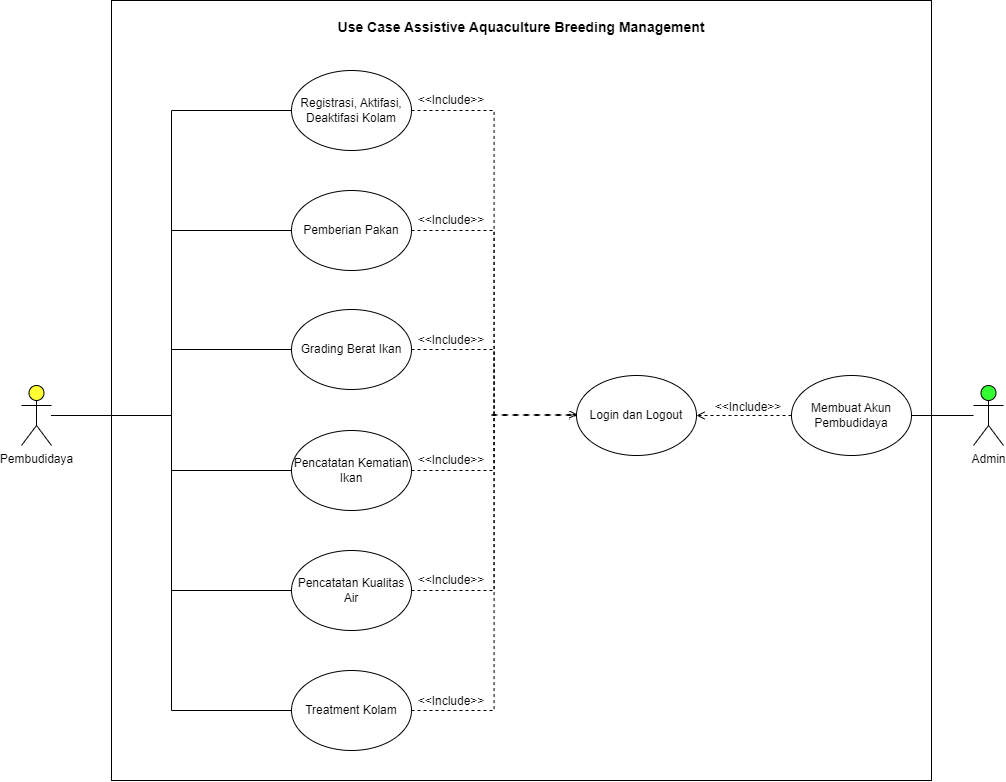
\includegraphics[keepaspectratio, width=13cm]{gambar/usecaseaquabreeding2}
	\caption{Use Case}
	\label{gambar:usecase}
\end{figure}

\section{Perancangan Sistem}

Metode perancangan sistem pada penelitian ini sesuai dengan komponen yang ada di dalam metode Scrum. Komponen-komponen tersebut terdiri dari \textit{product backlog}, \textit{sprint backlog}, \textit{sprint}, \textit{daily scrum}, dan \textit{pengujian sistem}. Aktivitas-aktivitas yang ditentukan digunakan di Scrum agar terciptanya keteraturan. Semua aktivitas dibatasi oleh waktu. Setelah Sprint dimulai, durasinya tetap dan tidak dapat dipersingkat atau diperpanjang. Aktivitas yang tersisa dapat berakhir setiap kali tujuan aktivitas tercapai, memastikan jumlah waktu yang tepat dihabiskan tanpa membiarkan pemborosan dalam proses. Aktivitas-aktivitas yang terdapat pada Scrum adalah Sprint, Sprint Planning, Daily Scrum, Sprint Review, Sprint Retrospective. tahapan dan aktivitas tersebut dapat dilihat pada gambar \ref{gambar:scrumflow}. 

\begin{figure}[H]
	\centering
	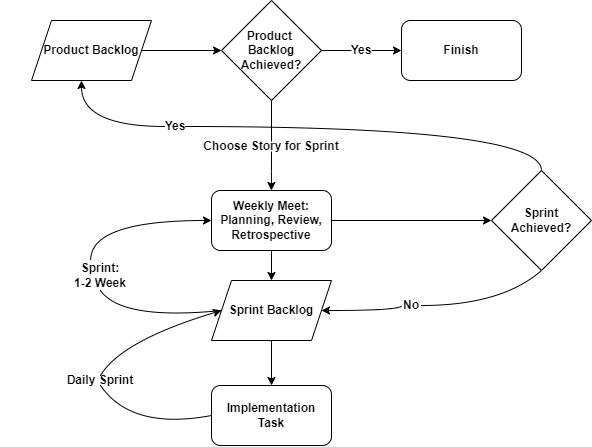
\includegraphics[keepaspectratio, width=11cm]{gambar/scrumflow}
	\caption{Tahapan dan aktivitas yang dilakukan dalam metode scrum}
	\label{gambar:scrumflow}
\end{figure}

\begin{enumerate}
\setlength{\enumerateparindent}{2em}
	\item{\textit{Product Backlog}}
	
	\hspace{\enumerateparindent} Tabel 3.1 merupakan tabel \textit{product backlog} aplikasi pendukung teknologi perikanan modern yang telah dibuat berdasarkan diskusi dengan \textit{Scrum Master}. Setiap \textit{item} dari \textit{product backlog} ini akan diimplementasikan pada \textit{sprint} dari awal hingga selesai.

\begin{table}[H]
	\caption{\textit{Product Backlog}}
	\label{product_backlog}
	\begin{tabular}{@{} |p{0.5cm}|p{8cm}|p{1.5cm}|p{2.5cm}| @{}}
		\hline
		\textbf{No} & \textbf{\textit{Story}} & \textbf{\textit{Sprint}} & \textbf{\textit{Status}} \\
		\hline
		1 & Membuat halaman dasboard & 1 & \\
		\hline
		2 & Membuat fitur registrasi kolam dan aktifasi Musim budidaya & 2 dan 3 & \\
		\hline
		3 & Membuat fitur pemberian pakan & 3 & \\
		\hline
		4 & Membuat fitur grading berat ikan perkolam & 4 & \\
		\hline
		5 & Membuat fitur pencatatan kematian & 5 & \\
		\hline
		6 & Membuat fitur treatmet kolam & 6 dan 7 & \\
		\hline
		7 & Membuat fitur pencatatan kualitas air harian &  8  & \\
		\hline
		8 & Membuat fitur pencatatan kualitas air mingguan & 9 & \\
		\hline
		9 & Membuat fitur perpindahan ikan antar kolam & 10 & \\
		\hline
		10 & Membuat fitur Multi User & 11 & \\
		\hline
	\end{tabular}
\end{table}

	\hspace{\enumerateparindent} Berdasarkan tabel \ref{product_backlog}, \textit{Product Backlog} pada penelitian ini terdiri dari 3 komponen, yaitu \textit{story}, \textit{sprint}, \textit{status}. \textit{Story} merupakan task besar yang nantinya akan dipecah lagi menjadi \textit{task-task} yang kecil di dalam \textit{Sprint}. Komponen \textit{sprint} pada tabel ini menandakan pada \textit{sprint} berapa \textit{story} tersebut akan dilaksanakan. Komponen \textit{status} menjelaskan apakah \textit{story} tersebut sudah selesai atau belum.

	\item{\textit{Sprint Backlog}}

	\hspace{\enumerateparindent} \textit{Sprint backlog} adalah daftar task yang perlu dikerjakan ataupun yang sudah dikerjakan pada \textit{sprint}. Di dalam \textit{sprint backlog}, berbagai \textit{task} kecil dibuat. Dengan Sprint Backlog, seluruh anggota tim dapat melihat perkembangan dari setiap pekerjaan.

	\item{\textit{Sprint}}

	\hspace{\enumerateparindent} Setelah dilakukan perencanaan pada Sprint Backlog, maka pengerjaan sprint sudah dapat dimulai dan harus mengikuti jadwal pengerjaan yang telah disepakati bersama tim. Dalam penelitian ini, interval sprint yang digunakan adalah satu sampai dua minggu.

	\item{\textit{Sprint Review} dan \textit{Sprint Retrospective}}

	\hspace{\enumerateparindent} \textit{Sprint review}, dan \textit{sprint retrospective} dilakukan pada setiap awal pekan yaitu di hari Selasa melalui \textit{voice call} menggunakan plaform discord dan juga tatap muka secara langsung. Pada awal pekan ini akan dilakukan evaluasi mengenai perkembangan proses pembuatan aplikasi maupun hambatan yang terjadi selama pengerjaan di setiap \textit{sprint}.

\end{enumerate}

\section{Pengujian Sistem}
Pada tahap ini peneliti akan melakukan uji aplikasi pendukung teknologi perikanan modern menggunakan dua jenis pengujian yaitu unit testing dan User Acceptance Test (UAT). Pengujian unit testing dilaksanakan oleh tim internal developer untuk memastikan fungsi-fungsi pada aplikasi yang telah dikembangkan dapat berjalan dengan baik. Sedangkan UAT dilaksanakan oleh pengguna dalam hal ini product owner yaitu UD Jfarm untuk mengetahui apakah aplikasi sudah sesuai kebutuhan dan layak digunakan.

\begin{enumerate}
\setlength{\enumerateparindent}{2em}
	\item{\textit{Unit Testing}}

	\hspace{\enumerateparindent} Skenario pada unit testing dibuat berdasarkan product backlog. Adapun skenario dari unit testing yang akan dilaksanakan terdapat pada tabel yang terdapat pada tabel dibawah ini.

\begin{longtable}[c]{@{} |p{4cm}|p{9.3cm}| @{}}
  \caption{Skenario \textit{Unit Testing} \label{unit_testing}}\\
 
  \hline
  \multicolumn{2}{| c |}{\textbf{Skenario \textit{Unit Testing}}}\\
  \hline
  \centering{\textbf{Uji Fitur}} & \centering{\textbf{Skenario Pengujian}}  
  \endfirsthead
 
  \hline
  \multicolumn{2}{| c |}{\textbf{Skenario \textit{Unit Testing}}}\\
  \hline
  \centering{\textbf{Uji Fitur}} & \centering{\textbf{Skenario Pengujian}}
  \endhead
 
  \hline
  \endfoot
 
  \hline
  \endlastfoot
 
  \hline
  Halaman Awal & Saat aplikasi dibuka akan muncul splash screen yang menampilkan logo yang menandakan aplikasi sedang loading\\
  \hline
   & Setelah loading selesai maka akan ditampikan halaman login\\
  \hline
  Login & Ketika mengisi form login dengan data yang sesuai kemudian menekan submit, maka akan masuk ke halaman dashboard\\
  \hline
   & Ketika mengisi form login dengan data yang tidak sesuai kemudian menekan submit, maka akan menampilkan pesan kesalahan\\
  \hline
  Halaman Dashboard & Saat ikon profil ditekan maka akan muncul halaman profil lembaga farm\\
  \hline
   & Saat tombol kolam ditekan maka akan muncul halaman yang menampilkan list kolam\\
  \hline
  Daftar Kolam & Saat ikon (+) ditekan maka akan menampilkan halaman registrasi kolam\\
  \hline
   & Saat card kolam ditekan akan menampilkan halaman detail kolam\\
  \hline
  Registrasi Kolam & ketika mengisi form registrasi kolam dengan data yang sesuai dan menekan submit, maka kolam baru akan ditambakan\\
  \hline
  Detail Kolam & ketika tombol kualitas air ditekan maka akan menampilkan halaman kualitas air\\
  \hline
   & ketikan menekan salah satu list dari masa budidaya akan menampilkan halaman detail masa budidaya\\
  \hline
   & ketika status kolam tidak aktif atau panen dan menekan tombol start budidaya, maka akan menampilkan halaman aktivasi kolam\\
  \hline
   & ketika status kolam aktif dan menekan tombol aktif, maka akan menampilkan halaman deaktivasi kolam\\
  \hline
  Aktivasi Kolam & ketika mengisi form aktivasi kolam dengan data yang sesuai dan menekan submit, maka musim budidaya baru akan ditambahkan dan status kolam menjadi aktif\\
  \hline
  Deaktivasi Kolam & ketika mengisi form deaktivasi kolam dengan data yang sesuai dan menekan submit, maka musim budidaya yang barjalan akan berhenti status kolam menjadi tidak aktif\\
  \hline
  Kualitas Air & Ketika memilih musim budidaya dan maka akan ditampilkan list pengontrolan kualitas air kolam\\
  \hline
   & Ketika menekan list data pengontrolan kualitas air, maka akan ditamplikan detail pengontrolan kualitas air kolam\\
  \hline
   & Saat ikon (+) ditekan maka akan menampilkan halaman entry pengontrolan kualitas air kolam\\
  \hline
   & ketika mengisi form pengontrolan kualitas air kolam dengan data yang sesuai dan menekan submit, data pengontrolan kualitas air akan ditambahkan\\
  \hline
  Detail Masa Budidaya & Ketika tombol rekapitulasi pakan ditekan, maka akan ditampilkan halaman rekapitulasi pakan\\
  \hline
   & Ketika tombol rekapitulasi kematian ikan ditekan, maka akan ditampilkan halaman rekapitulasi kematian ikan\\
  \hline
   & Ketika tombol rekapitulasi grading ikan ditekan, maka akan ditampilkan halaman rekapitulasi grading ikan\\
  \hline
   & Ketika tombol treatment ditekan, maka akan ditampilkan halaman treatment kolam\\
  \hline
   & Ketika tombol sortir ditekan, maka akan ditampilkan halaman sortir kolam\\
  \hline
   Rekapitulasi Pakan & Ketika menekan list data rekapitulasi pakan, maka akan ditamplikan detail rekapitulasi pakan\\
  \hline
   & Ketika menekan list data rekapitulasi pakan, maka akan ditamplikan detail rekapitulasi pakan\\
  \hline
   & Saat tombol entry pakan ditekan maka akan menampilkan halaman entry pakan\\
  \hline
    & ketika mengisi form rekapitulasi pakan dengan data yang sesuai dan menekan submit, data rekapitulasi pakan akan ditambahkan\\
  \hline
   Rekapitulasi Kematian & Ketika menekan list data rekapitulasi pakan, maka akan ditamplikan detail rekapitulasi pakan\\
  \hline
   & Saat tombol entry kematian ditekan maka akan menampilkan halaman entry kematian\\
  \hline
    & ketika mengisi form rekapitulasi kematian dengan data yang sesuai dan menekan submit, data rekapitulasi kematian akan ditambahkan\\
  \hline
   Rekapitulasi Grading & Ketika menekan list data rekapitulasi grading, maka akan ditamplikan detail rekapitulasi grading\\
  \hline
   & Ketika menekan list data rekapitulasi grading, maka akan ditamplikan detail rekapitulasi grading\\
  \hline
   & Saat tombol entry grading ditekan maka akan menampilkan halaman entry grading\\
  \hline
    & ketika mengisi form rekapitulasi grading dengan data yang sesuai dan menekan submit, data rekapitulasi grading akan ditambahkan\\
  \hline
   Halaman Treatment & Ketika menekan list data treatment, maka akan ditamplikan detail treatment\\
  \hline
   & Saat ikon (+) ditekan maka akan menampilkan halaman entry treatment\\
  \hline
    & ketika mengisi form treatment dengan data yang sesuai dan menekan submit, data treatment akan ditambahkan\\
  \hline
   Halaman Sortir & Ketika menekan list data sortir, maka akan ditamplikan detail sortir\\
  \hline
   & Saat ikon (+) ditekan maka akan menampilkan halaman entry sortir\\
  \hline
    & `\\
  \hline
  \end{longtable}

	\item{\textit{User Acceptance Test (UAT)}}

	\hspace{\enumerateparindent} User Acceptance Test dibuat berdasarkan fitur-fitur yang dapat diakses oleh pengguna pada product backlog. Adapun format dari UAT yang akan dilaksanakan terdapat pada tabel 3.3 dimana penulis menggunakan format yang digunakan oleh \citep{lee2018} sebagai referensi.


 \begin{longtable}[c]{@{} |p{1cm}|p{6.5cm}|p{1.1cm}|p{1.1cm}|p{1.1cm}|p{1.1cm}| @{}}
 \caption{Format \textit{User Acceptance Test} \label{user_testing}}\\

 \hline
 \multicolumn{6}{| c |}{\textbf{\textit{User Acceptance Test}}}\\
 \hline
  \multirow{2}{=}{\centering{\textbf{No}}} & \multirow{2}{=}{\centering{\textbf{\textit{Acceptance Requirements}}}} & \multicolumn{4}{| c |}{\textbf{Kesesuaian}}\\
 \cline{3-6}
   &  & \centering{\textbf{SS}} & \centering{\textbf{S}} & \centering{\textbf{TS}} & \centering{\textbf{STS}}
 \endfirsthead

 \hline
 \multicolumn{6}{| c |}{\textbf{\textit{User Acceptance Test}}}\\
 \hline
  \multirow{2}{=}{\centering{\textbf{No}}} & \multirow{2}{=}{\centering{\textbf{\textit{Acceptance Requirements}}}} & \multicolumn{4}{| c |}{\textbf{Kesesuaian}}\\
 \cline{3-6}
  &  & \centering{\textbf{SS}} & \centering{\textbf{S}} & \centering{\textbf{TS}} & \centering{\textbf{STS}}
 \endhead

 \hline
 \endfoot

 \hline
 \endlastfoot

 \hline
 1 & Fitur login sudah sesuai dengan kebutuhan pembudidaya &  &  &  &\\
 \hline
 2 & Fitur dasboard sudah sesuai dengan kebutuhan pembudidaya &  &  &  &\\
 \hline
 3 & Fitur registrasi, aktivasi dan deaktivasi sudah sesuai dengan kebutuhan pembudidaya &  &  &  &\\
 \hline
 4 & Fitur pemberian dan rekapitulasi pakan sudah sesuai dengan kebutuhan pembudidaya &  &  &  &\\
 \hline
 5 & Fitur grading berat ikan sudah sesuai dengan kebutuhan pembudidaya &  &  &  &\\
 \hline
 6 & Fitur pencatatan kematian sudah sesuai dengan kebutuhan pembudidaya &  &  &  &\\
 \hline
 7 & Fitur treatment kolam sudah sesuai dengan kebutuhan pembudidaya &  &  &  &\\
 \hline
 8 & Fitur pencatatan kualitas air harian sudah sesuai dengan kebutuhan pembudidaya &  &  &  &\\
 \hline
 9 & Fitur pencatatan kualitas air mingguan sudah sesuai dengan kebutuhan pembudidaya &  &  &  &\\
 \hline
 10 & Fitur sortir ikan sudah sesuai dengan kebutuhan pembudidaya &  &  &  &\\
 \hline
 \end{longtable}


\end{enumerate}

%\subsection{\textit{Daily Scrum}}

%Pada akhir pekan di akhir setiap \textit{sprint}, akan diadakan \textit{voice call} untuk membahas perkembangan dan hambatan pada setiap \textit{sprint}.